\chapter{Branden: wat een vuur nodig heeft}\label{ch:g4:what-a-fire-needs}

Een kampvuur in de schemering. Er was droog hout voor nodig en een
lucifer om het aan te steken, en de wind die erdoorheen waait, houdt het
fel. Na een uur zijn de blokken geslonken tot gloeiende sintels en witte
as, en is er grijze rook naar de \omterm{def:g4:air-a-mixture-of-gases:air}{lucht} weggedreven. Waar is het hout
gebleven? Wat heeft een vuur nodig, en wat laat het achter?

\begin{recall}
\omterm{def:g4:air-a-mixture-of-gases:air}{Lucht} is een mengsel van gassen: ongeveer vier vijfde stikstof en een
vijfde zuurstof, met een beetje argon en koolstofdioxide. Een vlam haalt
zuurstof uit de \omterm{def:g4:air-a-mixture-of-gases:air}{lucht} om zich heen; een kaars onder een stolp gaat uit
als er te weinig zuurstof over is (\cref{ch:g4:air-a-mixture-of-gases}).
\end{recall}

\begin{omfigure}
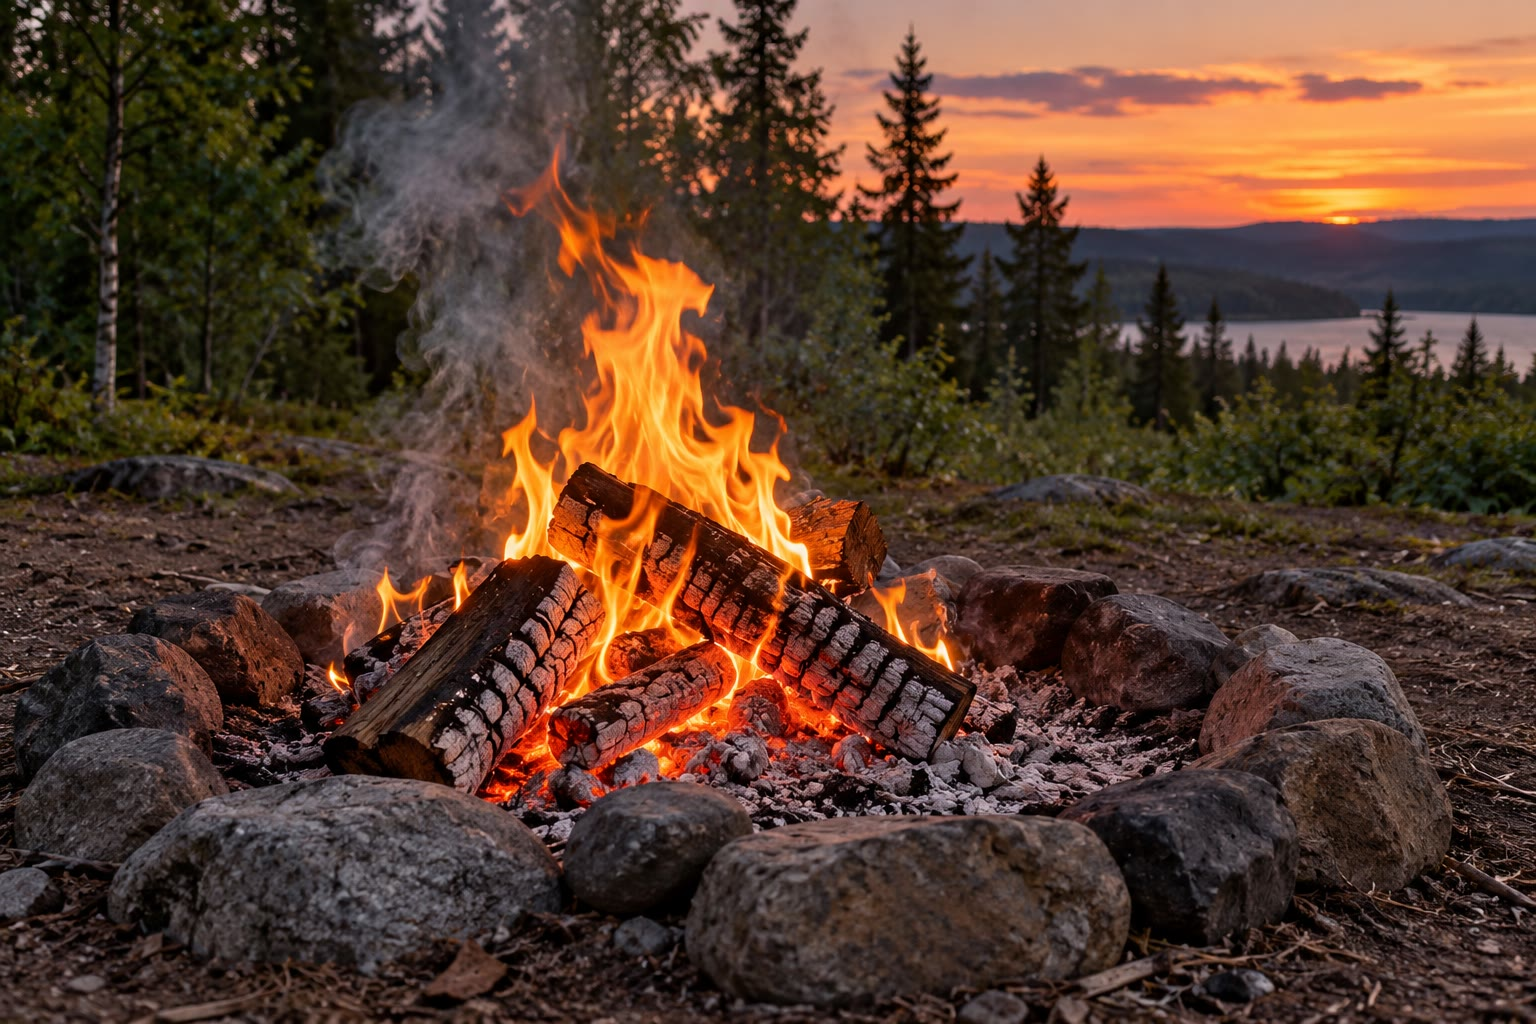
\includegraphics[width=0.6\linewidth]{images/book1/ai/g4-campfire.jpg}

{\small Een kampvuur: hout, \omterm{def:g4:air-a-mixture-of-gases:air}{lucht} en een lucifer --- en na afloop as en
rook.}
\end{omfigure}

\section{Brandstoffen}

\begin{definition}[Brandstof]\label{def:g4:what-a-fire-needs:fuel}
Een \emph{brandstof}\index{brandstof} is een materiaal dat kan \omterm{def:g4:what-a-fire-needs:burning}{branden}
en daarbij warmte en licht geeft: hout, papier, steenkool, kaarsvet, het
gas van een fornuis, benzine, stookolie.
\end{definition}

\begin{example}[Vaste, vloeibare en gasvormige brandstoffen]\label{ex:g4:what-a-fire-needs:fuels}
Hout, papier, steenkool en kaarsvet zijn vaste \omterm{def:g4:what-a-fire-needs:fuel}{brandstoffen}. Benzine en
stookolie zijn vloeibare \omterm{def:g4:what-a-fire-needs:fuel}{brandstoffen}. Het gas van een gasfornuis en het
gas in een aansteker zijn gasvormige \omterm{def:g4:what-a-fire-needs:fuel}{brandstoffen}.
\end{example}

\begin{remark}[Niet alles brandt]\label{rem:g4:what-a-fire-needs:not}
Steen, zand, glas en water \omterm{def:g4:what-a-fire-needs:burning}{branden} niet: het zijn geen \omterm{def:g4:what-a-fire-needs:fuel}{brandstoffen}.
Daarom bouw je een open haard van steen of baksteen, en daarom gebruik
je zand en water om een brand te blussen.
\end{remark}

\section{De branddriehoek}

\begin{definition}[Branddriehoek]\label{def:g4:what-a-fire-needs:fire-triangle}
Een vuur heeft drie dingen tegelijk nodig: een \omterm{def:g4:what-a-fire-needs:fuel}{brandstof}, zuurstof uit de
\omterm{def:g4:air-a-mixture-of-gases:air}{lucht}, en warmte om het aan te steken. Die drie dingen tekenen we als de
drie zijden van een driehoek, de
\emph{branddriehoek}\index{branddriehoek}. Ontbreekt er één zijde, dan is
er geen vuur.
\end{definition}

\begin{omfigure}
\begin{tikzpicture}[font=\small]
  \coordinate (A) at (0,0); \coordinate (B) at (5,0); \coordinate (C) at (2.5,4.1);
  \draw[line width=3pt, brown!70!black] (A) -- (B);
  \draw[line width=3pt, omDef] (B) -- (C);
  \draw[line width=3pt, red!75!black] (C) -- (A);
  \node[below=4pt, font=\small\bfseries, brown!60!black] at (2.5,0) {brandstof};
  \node[right=4pt, font=\small\bfseries, omDef] at (3.75,2.05) {zuurstof (uit de lucht)};
  \node[left=4pt, font=\small\bfseries, red!75!black] at (1.25,2.05) {warmte (om aan te steken)};
  % a flame in the middle
  \fill[orange!80] (2.5,0.55) .. controls (1.95,1.15) and (2.35,1.75) .. (2.55,2.3)
    .. controls (2.75,1.75) and (3.05,1.15) .. (2.5,0.55);
  \fill[yellow!80] (2.5,0.7) .. controls (2.25,1.05) and (2.4,1.35) .. (2.52,1.65)
    .. controls (2.62,1.35) and (2.75,1.05) .. (2.5,0.7);
\end{tikzpicture}

{\small De \omterm{def:g4:what-a-fire-needs:fire-triangle}{branddriehoek}: \omterm{def:g4:what-a-fire-needs:fuel}{brandstof}, zuurstof en warmte, alle drie
tegelijk.}
\end{omfigure}

\begin{example}[Een lucifer aansteken]\label{ex:g4:what-a-fire-needs:match}
Je strijkt de kop van een lucifer langs de zijkant van het doosje. Door
het wrijven wordt hij zo warm dat hij begint te \omterm{def:g4:what-a-fire-needs:burning}{branden}: dat is de
warmtezijde van de driehoek. Het hout van de lucifer is de \omterm{def:g4:what-a-fire-needs:fuel}{brandstof}, en
de \omterm{def:g4:air-a-mixture-of-gases:air}{lucht} brengt de zuurstof.
\end{example}

\begin{example}[Op sintels blazen]\label{ex:g4:what-a-fire-needs:embers}
Gloeiende sintels die bijna uit lijken, laaien weer op als iemand erop
blaast: het blazen brengt meer \omterm{def:g4:air-a-mixture-of-gases:air}{lucht}, en dus meer zuurstof, bij de
\omterm{def:g4:what-a-fire-needs:fuel}{brandstof} die nog heet is.
\end{example}

\section{Bij branden ontstaan nieuwe stoffen}

\begin{definition}[Branden en verbranding]\label{def:g4:what-a-fire-needs:burning}
\emph{Branden}\index{branden} is wat er gebeurt als een \omterm{def:g4:what-a-fire-needs:fuel}{brandstof}
zuurstof uit de \omterm{def:g4:air-a-mixture-of-gases:air}{lucht} opneemt en warmte en licht geeft. Scheikundigen
noemen dat branden een \emph{verbranding}\index{verbranding}. Bij een
verbranding worden de \omterm{def:g4:what-a-fire-needs:fuel}{brandstof} en de zuurstof verbruikt, en ontstaan er
nieuwe stoffen: rook, as, koolstofdioxide en waterdamp.
\end{definition}

\begin{proposition}[Een verbranding is niet terug te draaien]\label{prop:g4:what-a-fire-needs:new}
De as en de rook van een vuur worden nooit meer hout, hoe lang we ook
wachten. Bij \omterm{def:g4:what-a-fire-needs:burning}{branden} ontstaan nieuwe stoffen die er eerst niet waren; de
\omterm{def:g4:what-a-fire-needs:fuel}{brandstof} is voorgoed weg.
\end{proposition}

\begin{inthelab}[Een koud glas boven een kaars]
De docent houdt een koud, droog bekerglas even ondersteboven boven een
kaarsvlam. De binnenkant van het glas beslaat met piepkleine
waterdruppeltjes: waterdamp die de brandende kaars maakt, is op het koude
glas weer vloeibaar geworden. Een brandende kaars maakt water, en ook
koolstofdioxide, dat je kunt aantonen met een test uit een later
hoofdstuk.
\end{inthelab}

\begin{omfigure}
\begin{tikzpicture}[font=\small, scale=1.3]
  % candle
  \fill[white, draw=black!50] (-0.25,0) rectangle (0.25,1.2);
  \draw[black!70] (0,1.2) -- (0,1.33);
  \fill[orange!85] (0,1.3) .. controls (-0.16,1.5) and (-0.06,1.75) .. (0,1.95)
    .. controls (0.06,1.75) and (0.16,1.5) .. (0,1.3);
  \fill[yellow!85] (0,1.36) .. controls (-0.08,1.5) and (-0.03,1.62) .. (0,1.72)
    .. controls (0.03,1.62) and (0.08,1.5) .. (0,1.36);
  % upturned cold beaker above
  \pic[transform shape, rotate=180] at (0,4.3) {beaker={0}{white}};
  \foreach \x/\y in {-0.6/3.9,-0.45/4.1,-0.2/3.95,0.1/4.15,0.35/3.9,0.6/4.05,
                     -0.7/3.5,0.7/3.4,-0.72/3.0,0.72/2.9}
    \fill[omDef!55] (\x,\y) circle (0.035);
  \draw[<-, omProp, thick] (0.68,3.95) -- (2.0,4.2) node[right, text=black]
    {waterdruppeltjes};
  \draw[<-, omProp, thick] (0.85,3.2) -- (2.0,3.3) node[right, text=black]
    {koud glas, ondersteboven};
  \draw[<-, omProp, thick] (0.15,1.7) -- (2.0,1.9) node[right, text=black]
    {de vlam: brandend kaarsvet};
  \draw[<-, omProp, thick] (0.3,0.6) -- (2.0,0.7) node[right, text=black]
    {kaarsvet: de brandstof};
\end{tikzpicture}

{\small Een koud glas boven een kaars beslaat: brandend kaarsvet maakt
waterdamp.}
\end{omfigure}

\begin{example}[Wat een houtblok wordt]\label{ex:g4:what-a-fire-needs:log}
Een houtblok van een paar kilo brandt op tot een hoopje as. Het meeste
hout is niet verdwenen: samen met zuurstof uit de \omterm{def:g4:air-a-mixture-of-gases:air}{lucht} is het rook,
koolstofdioxide en waterdamp geworden, en dat zijn gassen die naar de
\omterm{def:g4:air-a-mixture-of-gases:air}{lucht} wegdrijven.
\end{example}

\section{Een vuur blussen}

\begin{method}[Een vuur blussen: haal één zijde weg]\label{met:g4:what-a-fire-needs:out}
Om een vuur te blussen, haal je één zijde van de \omterm{def:g4:what-a-fire-needs:fire-triangle}{branddriehoek} weg:
\begin{itemize}
  \item \textbf{haal de zuurstof weg}: bedek het vuur met een
        blusdeken, een deksel of zand, zodat er geen \omterm{def:g4:air-a-mixture-of-gases:air}{lucht} bij kan;
  \item \textbf{haal de warmte weg}: giet water op brandend hout of
        papier; dat koelt het af tot onder de temperatuur waarbij het kan
        \omterm{def:g4:what-a-fire-needs:burning}{branden};
  \item \textbf{haal de \omterm{def:g4:what-a-fire-needs:fuel}{brandstof} weg}: draai de gaskraan dicht, of haal
        bij een bosbrand de droge planten rond het vuur weg.
\end{itemize}
\end{method}

\begin{omfigure}
\begin{tikzpicture}[font=\small, scale=0.7]
  \foreach \k/\lab/\side in {0/{een deken: geen zuurstof}/1, 1/{water: geen warmte}/2,
                              2/{gas dicht: geen brandstof}/0} {
    \begin{scope}[xshift=\k*6.2cm]
      \coordinate (A) at (0,0); \coordinate (B) at (4,0); \coordinate (C) at (2,3.3);
      \pgfmathsetmacro\oa{\side==0 ? 0.2 : 1}
      \pgfmathsetmacro\ob{\side==1 ? 0.2 : 1}
      \pgfmathsetmacro\oc{\side==2 ? 0.2 : 1}
      \draw[line width=2.5pt, brown!70!black, opacity=\oa] (A) -- (B);
      \draw[line width=2.5pt, omDef, opacity=\ob] (B) -- (C);
      \draw[line width=2.5pt, red!75!black, opacity=\oc] (C) -- (A);
      \ifnum\side=0 \draw[line width=1.4pt, black] (1.6,-0.4) -- (2.4,0.4) (1.6,0.4) -- (2.4,-0.4);\fi
      \ifnum\side=1 \draw[line width=1.4pt, black] (2.6,1.25) -- (3.4,2.05) (2.6,2.05) -- (3.4,1.25);\fi
      \ifnum\side=2 \draw[line width=1.4pt, black] (0.6,1.25) -- (1.4,2.05) (0.6,2.05) -- (1.4,1.25);\fi
      \node[align=center, anchor=north] at (2,-0.6) {\lab};
    \end{scope}
  }
\end{tikzpicture}

{\small Drie manieren om een vuur te blussen, die elk één zijde van de
driehoek weghalen (doorgekruist): de zuurstof, de warmte of de
\omterm{def:g4:what-a-fire-needs:fuel}{brandstof}.}
\end{omfigure}

\begin{omfigure}
\begin{minipage}[t]{0.48\linewidth}\centering
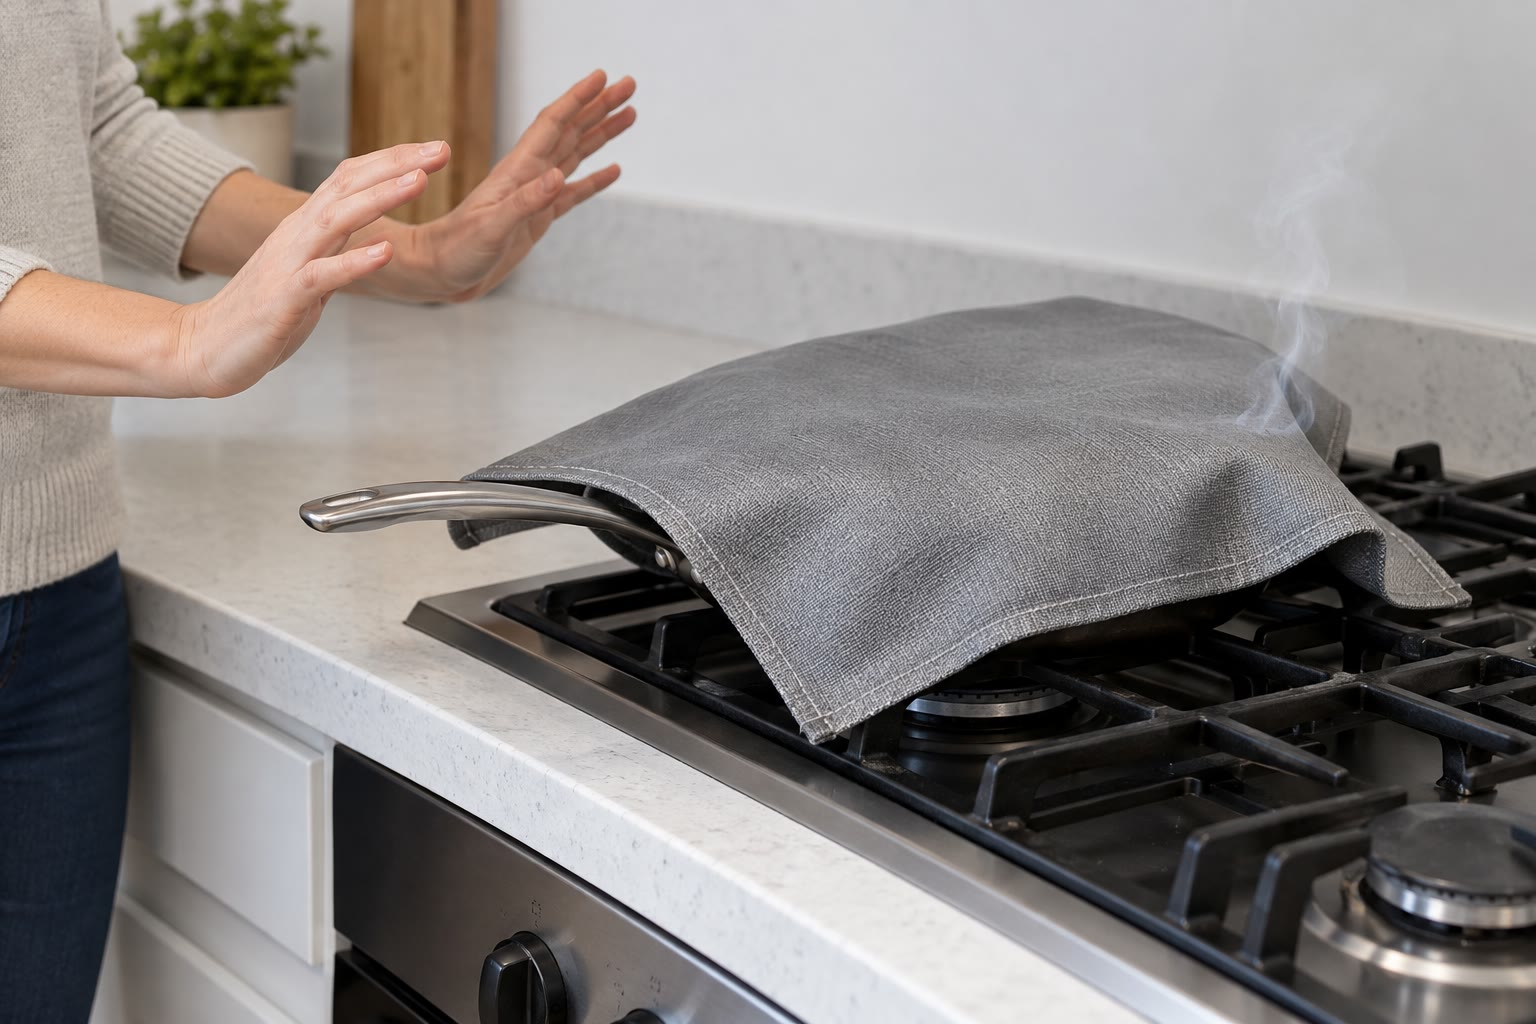
\includegraphics[width=\linewidth,height=4.6cm,keepaspectratio]{images/book1/ai/g4-fire-blanket.jpg}

{\small Een blusdeken over een pan: de \omterm{def:g4:air-a-mixture-of-gases:air}{lucht} kan het vuur niet meer
bereiken.}
\end{minipage}\hfill
\begin{minipage}[t]{0.48\linewidth}\centering
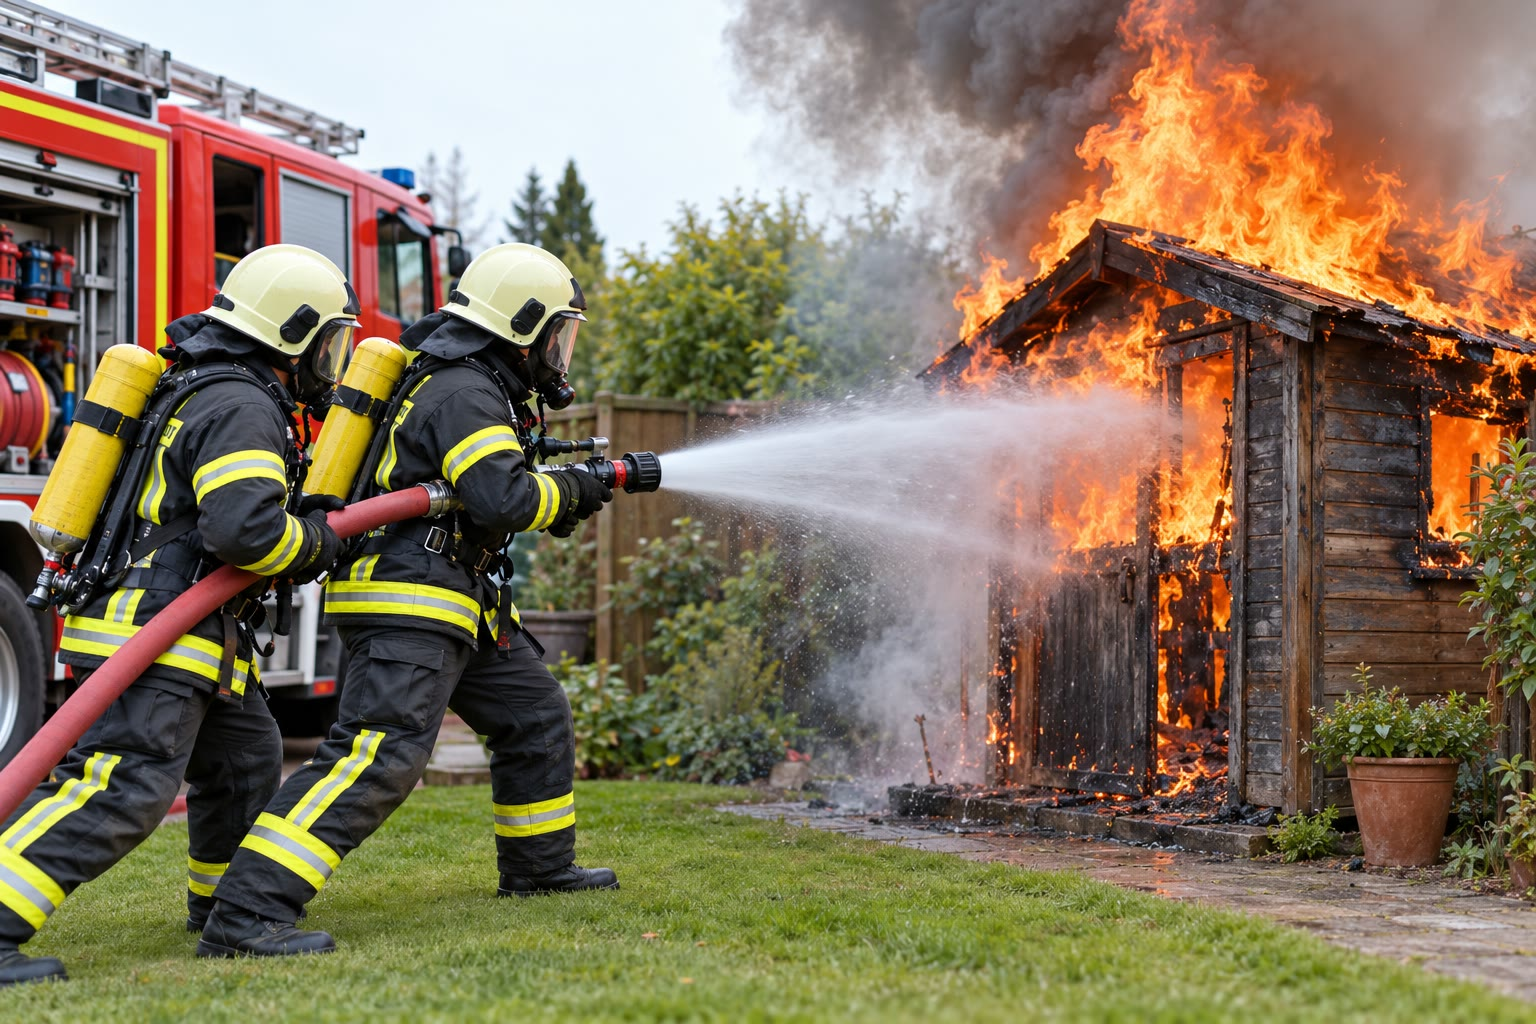
\includegraphics[width=\linewidth,height=4.6cm,keepaspectratio]{images/book1/ai/g4-firefighters.jpg}

{\small Brandweerlieden spuiten water om een brandende schuur af te
koelen.}
\end{minipage}
\end{omfigure}

\section{Brandveiligheid}

\begin{remark}[Nooit water op een pan brandende olie]\label{rem:g4:what-a-fire-needs:oil}
Als de olie in een koekenpan vlam vat, mag niemand er water op gooien:
het water kookt meteen onder de olie en slingert brandende olie uit de
pan. Een volwassene draait het gas of de kookplaat uit en dekt de pan af
met een deksel of een blusdeken.
\end{remark}

\begin{safety}{\ghs{GHS02}\ghs{GHS04}}
% ledger: ghs:butane
Het gas in een aansteker of een kampeergasbusje is butaan. Het
vlammenpictogram (GHS02) betekent: zeer licht ontvlambaar, uit de buurt
houden van vlammen en vonken. Het pictogram met de gasfles (GHS04)
betekent: een gas dat onder druk staat.
\end{safety}

\begin{proposition}[Wat je doet als er brand is]\label{prop:g4:what-a-fire-needs:safety}
Rook is het eerste gevaar van een brand: hij is heet, hij verbergt de
uitgang en het is giftig om hem in te ademen. Een rookmelder aan het
plafond piept luid zodra er rook bij komt. Als er brand is: ga naar
buiten, blijf laag onder de rook, doe de deuren achter je dicht en bel
de brandweer van buitenaf. Ga nooit meer naar binnen.
\end{proposition}

\begin{omfigure}
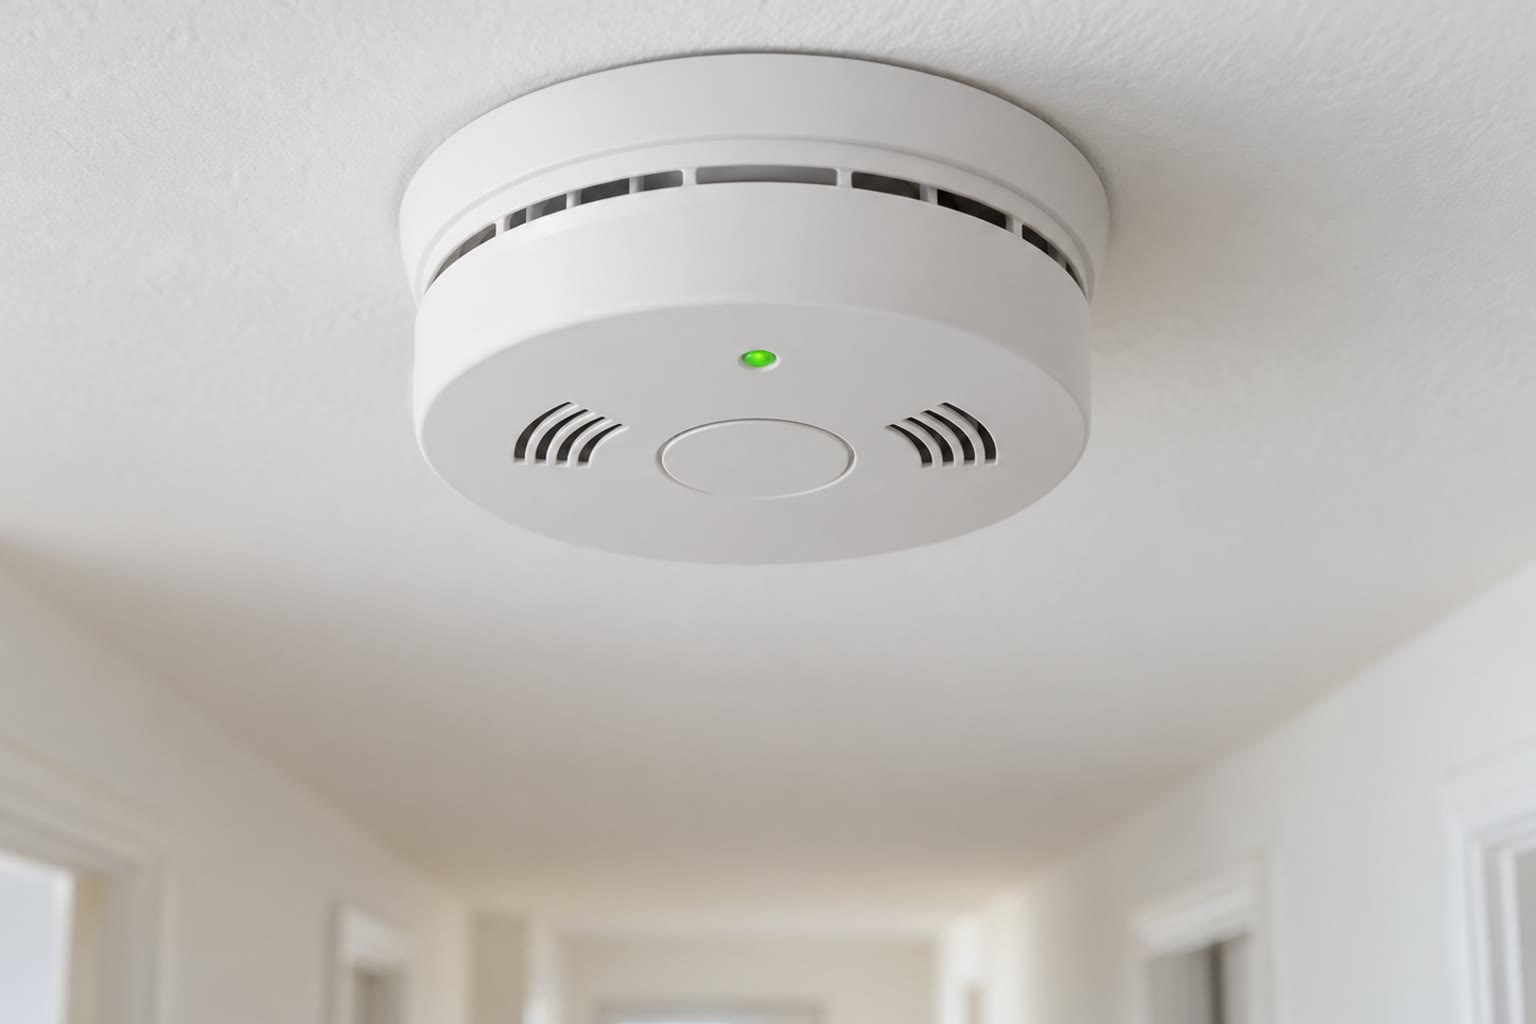
\includegraphics[width=0.42\linewidth]{images/book1/ai/g4-smoke-alarm.jpg}

{\small Een rookmelder: hij gaat af zodra er rook bij komt.}
\end{omfigure}

\section{Oefeningen}

\begin{exercise}[$\star$]\label{exo:g4:what-a-fire-needs:1}
Noem de drie zijden van de \omterm{def:g4:what-a-fire-needs:fire-triangle}{branddriehoek}.
\end{exercise}

\begin{exercise}[$\star$]\label{exo:g4:what-a-fire-needs:2}
Welke hiervan zijn \omterm{def:g4:what-a-fire-needs:fuel}{brandstoffen}: hout, zand, kaarsvet, glas, benzine,
water, papier?
\end{exercise}

\begin{exercise}[$\star$]\label{exo:g4:what-a-fire-needs:3}
Over een klein vuur wordt een blusdeken gegooid. Welke zijde van de
\omterm{def:g4:what-a-fire-needs:fire-triangle}{branddriehoek} haalt die weg?
\end{exercise}

\begin{exercise}[$\star$]\label{exo:g4:what-a-fire-needs:4}
Brandweerlieden spuiten water op een brandende schuur. Welke zijde van de
\omterm{def:g4:what-a-fire-needs:fire-triangle}{branddriehoek} haalt het water weg?
\end{exercise}

\begin{exercise}[$\star$]\label{exo:g4:what-a-fire-needs:5}
Noem drie nieuwe stoffen die ontstaan als hout brandt.
\end{exercise}

\begin{exercise}[$\star$]\label{exo:g4:what-a-fire-needs:6}
Waarom laaien gloeiende sintels weer op als je erop blaast?
\end{exercise}

\begin{exercise}[$\star$]\label{exo:g4:what-a-fire-needs:7}
Een koud glas boven een kaars beslaat. Welke nieuwe stof heeft de kaars
gemaakt?
\end{exercise}

\begin{exercise}[$\star$]\label{exo:g4:what-a-fire-needs:8}
Wat doe je eerst als een rookmelder afgaat en je rook ziet?
\end{exercise}

\begin{exercise}[$\star$]\label{exo:g4:what-a-fire-needs:9}
Kijk naar de figuur met de drie kleine driehoeken. Welke zijde is
doorgekruist als het gas dicht is gedraaid?
\end{exercise}

\begin{exercise}[$\star\star$]\label{exo:g4:what-a-fire-needs:10}
Om een bosbrand te stoppen, kappen brandweerlieden soms een brede strook
bomen vóór het vuur. Welke zijde van de \omterm{def:g4:what-a-fire-needs:fire-triangle}{branddriehoek} halen ze weg?
\end{exercise}

\begin{exercise}[$\star\star$]\label{exo:g4:what-a-fire-needs:11}
Een houtblok weegt veel meer dan zijn as. Is een deel van het houtblok
verdwenen? Leg uit waar het gebleven is.
\end{exercise}
